\documentclass[
11pt, % The default document font size, options: 10pt, 11pt, 12pt
%codirector, % Uncomment to add a codirector to the title page
]{charter} 


% El títulos de la memoria, se usa en la carátula y se puede usar el cualquier lugar del documento con el comando \ttitle
\titulo{KiwiScan: Sistema embebido para inspección de plantaciones de kiwis} 

% Nombre del posgrado, se usa en la carátula y se puede usar el cualquier lugar del documento con el comando \degreename
\posgrado{Carrera de Especialización en Sistemas Embebidos} 
%\posgrado{Carrera de Especialización en Internet de las Cosas} 
%\posgrado{Carrera de Especialización en Inteligencia Artificial}
%\posgrado{Maestría en Sistemas Embebidos} 
%\posgrado{Maestría en Internet de las cosas}
% IMPORTANTE: no omitir titulaciones ni tildación en los nombres, también se recomienda escribir los nombres completos (tal cual los tienen en su documento)
% Tu nombre, se puede usar el cualquier lugar del documento con el comando \authorname
\autor{Lic. Dante Mendoza}

% El nombre del director y co-director, se puede usar el cualquier lugar del documento con el comando \supname y \cosupname y \pertesupname y \pertecosupname
\director{Esp. Ing. Roberto Guglielmino}
\pertenenciaDirector{UNO} 
\codirector{} % para que aparezca en la portada se debe descomentar la opción codirector en los parámetros de documentclass
\pertenenciaCoDirector{FIUBA}

% Nombre del cliente, quien va a aprobar los resultados del proyecto, se puede usar con el comando \clientename y \empclientename
\cliente{Universidad Nacional del Oeste}
\empresaCliente{UNO}
 
\fechaINICIO{23 de abril de 2024}		%Fecha de inicio de la cursada de GdP \fechaInicioName
\fechaFINALPlan{11 de junio de 2024} 	%Fecha de final de cursada de GdP
\fechaFINALTrabajo{18 de diciembre de 2024}	%Fecha de defensa pública del trabajo final


\begin{document}

\maketitle
\thispagestyle{empty}
\pagebreak


\thispagestyle{empty}
{\setlength{\parskip}{0pt}
\tableofcontents{}
}
\pagebreak


\section*{Registros de cambios}
\label{sec:registro}


\begin{table}[ht]
\label{tab:registro}
\centering
\begin{tabularx}{\linewidth}{@{}|c|X|c|@{}}
\hline
\rowcolor[HTML]{C0C0C0} 
Revisión & \multicolumn{1}{c|}{\cellcolor[HTML]{C0C0C0}Detalles de los cambios realizados} & Fecha      \\ \hline
0      & Creación del documento                                 &\fechaInicioName \\ \hline
1      & Se completa hasta el punto 5 inclusive                & {7} de {mayo} de 2024 \\ \hline
2      & Se completa hasta el punto 9 inclusive
%		  Se puede agregar algo más \newline
%		  En distintas líneas \newline
                                                 & {14} de {mayo} de 2024 \\ \hline
3      & Se completa hasta el punto 12 inclusive                & {21} de {mayo} de 2024 \\ \hline
4      & Se completa el plan	                                 & {28} de {mayo} de 2024 \\ \hline

% Si hay más correcciones pasada la versión 4 también se deben especificar acá

\end{tabularx}
\end{table}

\pagebreak



\section*{Acta de constitución del proyecto}
\label{sec:acta}

\begin{flushright}
Buenos Aires, \fechaInicioName
\end{flushright}

\vspace{2cm}

Por medio de la presente se acuerda con el \authorname\hspace{1px} que su Trabajo Final de la \degreename\hspace{1px} se titulará ``\ttitle'' y consistirá en la implementación de un prototipo de un sistema de inspección de plantaciones. El trabajo tendrá un presupuesto preliminar estimado de 725 horas y un costo estimado de \$ 33.325.750 pesos argentinos (ARS), con fecha de inicio el \fechaInicioName\hspace{1px} y fecha de presentación pública el \fechaFinalName.

Se adjunta a esta acta la planificación inicial.

\vfill

% Esta parte se construye sola con la información que hayan cargado en el preámbulo del documento y no debe modificarla
\begin{table}[ht]
\centering
\begin{tabular}{ccc}
\begin{tabular}[c]{@{}c@{}}Dr. Ing. Ariel Lutenberg \\ Director posgrado FIUBA\end{tabular} & \hspace{2cm} & \begin{tabular}[c]{@{}c@{}}\clientename \\ \empclientename \end{tabular} \vspace{2.5cm} \\ 
\multicolumn{3}{c}{\begin{tabular}[c]{@{}c@{}} \supname \\ Director del Trabajo Final\end{tabular}} \vspace{2.5cm} \\
\end{tabular}
\end{table}




\section{1. Descripción técnica-conceptual del proyecto a realizar}
\label{sec:descripcion}

En la Argentina la actividad relacionada con la cosecha del kiwi es una de las que ganó más relevancia en las últimas décadas, donde maximizar las ganancias es crucial para que sea una actividad redituable. 

Actualmente, se estima el volumen de cosecha contando los frutos por unidad de superficie en una etapa avanzada de desarrollo. Sin embargo, esta estimación tardía es demasiado cercana a la cosecha y muy dificultosa en plantaciones medianas a grandes. Una estimación temprana del rendimiento permitiría tomar decisiones operativas y estratégicas. Desde el punto de vista operativo, podría orientar en cuál será la necesidad de recursos permitiendo un uso más racional de los mismos y desde el punto de vista estratégico, posibilitará anticipar la negociación de la producción en el mercado interno o externo.

Por lo tanto, el objetivo de este proyecto es desarrollar un prototipo equipado con cámaras, sensores ultrasónicos, pantalla LCD, lector de tarjetas microSD, temperatura y humedad. Este se encontrará montado en un medio de transporte adecuado a las características de la plantación. Dicho prototipo permitirá la captura automatizada de imágenes de los frutos en la plantación, así como el registro de datos ambientales relevantes durante el recorrido. Los datos se almacenarán localmente en la tarjeta microSD. Posteriormente, mediante técnicas de visión por computadora, se procesarán las imágenes para detectar objetos relevantes, como frutos en estado temprano de maduración. 

Finalmente, la información sobre los totales detectados y los datos meteorológicos será guardada en un archivo de texto plano. Por lo tanto, se proporciona al productor información valiosa para la toma de decisiones respecto a la planificación y ejecución de la cosecha. En la figura \ref{fig:diagBloques}, se puede apreciar un diagrama de bloques del prototipo. 

\begin{figure}[htpb]
\centering 
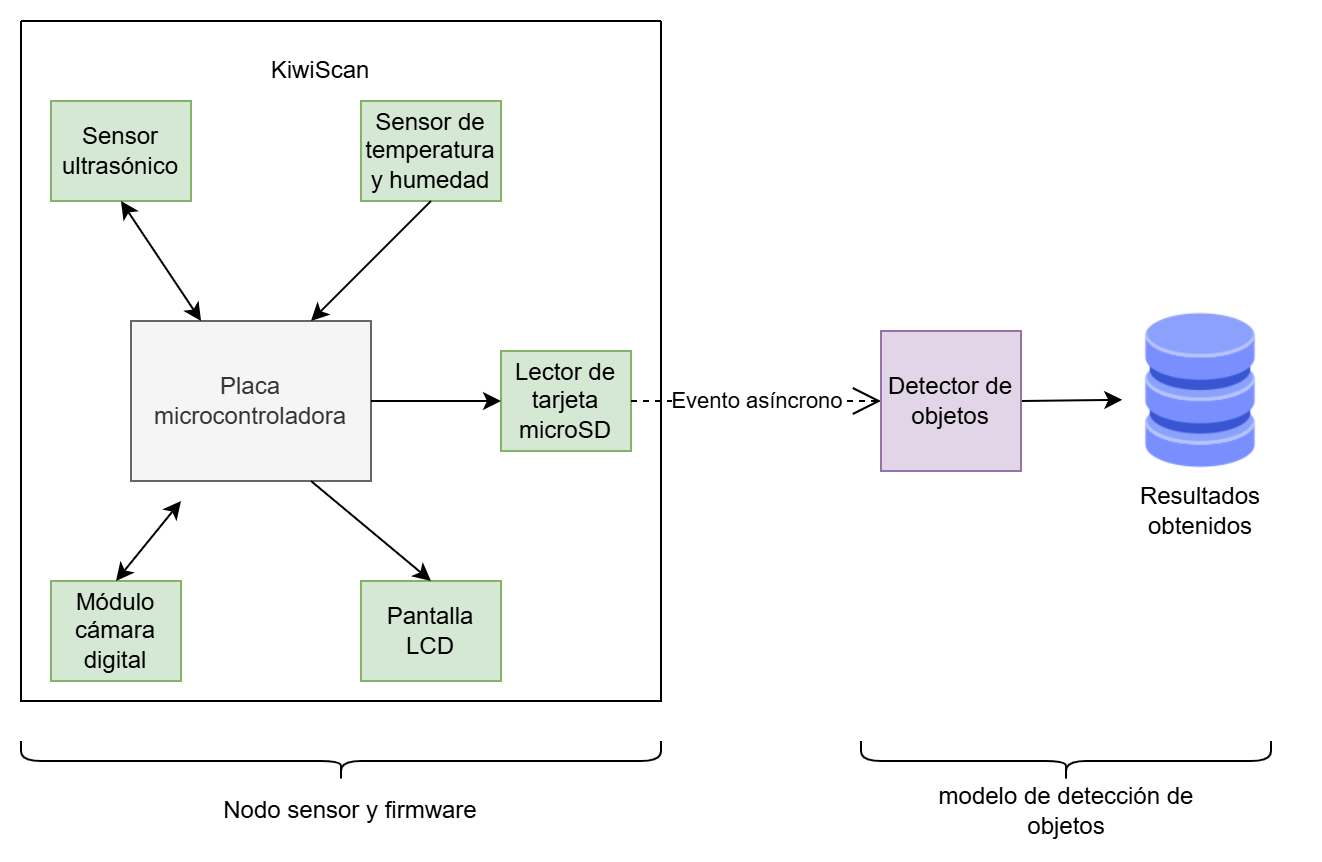
\includegraphics[width=.90\textwidth]{./Figuras/KiwiScan.png}
\caption{Diagrama en bloques del sistema.}
\label{fig:diagBloques}
\end{figure}

\vspace{10px}


\section{2. Identificación y análisis de los interesados}
\label{sec:interesados}

En este apartado, se definirán los involucrados dentro del presente proyecto;

\begin{table}[ht]
%\caption{Identificación de los interesados}
%\label{tab:interesados}
\begin{tabularx}{\linewidth}{@{}|l|X|X|l|@{}}
\hline
\rowcolor[HTML]{C0C0C0} 
Rol           & Nombre y Apellido & Organización 	& Puesto 	\\ \hline
Cliente       & \clientename      &\empclientename	& -       	\\ \hline
Responsable   & \authorname       & FIUBA        	& Alumno 	\\ \hline
Colaboradores & Lic. Aldana Ojeda  & -            & Investigadora       	\\ \hline
Orientador    & \supname	      & \pertesupname 	& Director del Trabajo Final \\ \hline
Usuario final   & Agricultores	      & - 	& - \\ \hline
\end{tabularx}
\end{table}

Por lo tanto, es importante destacar algunas características de los involucrados mencionados;

\begin{itemize}
	\item Orientador: \supname\hspace{1px} es experto en la temática y va a ayudar con la definición de los requerimientos y el desarrollo del firmware del embebido.
	\item Colaboradores: Lic. Aldana Ojeda es investigadora ad honorem con experiencia en el área.
    \item Cliente: La universidad UNO es la principal interesada en llevar a cabo este trabajo de investigación.
    \item Usuario final: Los agricultores serán los beneficiarios de la implementación.
    \item Responsable: Será quien dispondrá del conocimiento y desarrollo del proyecto.
\end{itemize}


\section{3. Propósito del proyecto}
\label{sec:proposito}

La importancia de este proyecto radica en su capacidad para acelerar el proceso de inspección de las plantaciones de kiwis, ofreciendo una alternativa eficaz a los métodos manuales convencionales. Esto se traduce en una mayor certeza en cuanto a la producción y una optimización de los recursos para los productores.

\section{4. Alcance del proyecto}
\label{sec:alcance}

El proyecto incluye:
\begin{itemize}
    \item Desarrollo de un prototipo funcional.
    \item Desarrollo del firmware para el microcontrolador.
    \item Pruebas de funcionamiento.
\end{itemize}

\newpage

El proyecto no incluye:
\begin{itemize}
	\item Desarrollo del modelo de detección de objetos.
	\item Clasificación y toma de imágenes para entrenamiento del modelo.
    \item Diseño y fabricación del gabinete que alojará al prototipo.
    \item Manuales de instalación y de usuario del dispositivo.
\end{itemize}


\section{5. Supuestos del proyecto}
\label{sec:supuestos}

Para el desarrollo del presente proyecto, se estima que se dispondrá de los siguientes elementos o consideraciones:

\begin{itemize}
	\item Adquisición de sensores.
	\item Importación de módulos que no se consigan en el mercado local.
	\item Consultas a expertos en la plantación de kiwis.
    \item Horas hombre para la codificación.
    \item Reuniones con el equipo de trabajo.
    \item Equipamiento informático.
    \item Licencias de software.
    \item Artículos de librería.
    \item Pasajes y viáticos para visita a la plantación.
    \item El presupuesto no superará en gran medida lo estimado.
\end{itemize}


\section{6. Requerimientos}
\label{sec:requerimientos}
Esta sección detalla los requerimientos del software, delineando las funcionalidades y características necesarias para cumplir con los objetivos del proyecto.

\begin{enumerate}
	\item Requerimientos funcionales:
		\begin{enumerate}
			\item El sistema debe registrar la temperatura del ambiente.
			\item El sistema debe registrar la humedad del ambiente.
			\item El sistema debe informar el espacio disponible de la tarjeta microSD.
            \item El sistema debe informar la cantidad de fotos tomadas.
		\end{enumerate}
	\item Requerimientos no funcionales:
		\begin{enumerate}
			\item El sistema debe ser escalable, de forma de poder agregar más sensores en el futuro.
			\item El firmware debe estar modularizado.
            \item El firmware debe estar sobre un sistema operativo.
		\end{enumerate}
    \item Requerimientos de interfaz gráfica en la pantalla LCD:
		\begin{enumerate}
			\item Se debe mostrar los valores de humedad y temperatura.
			\item Se debe mostrar el espacio disponible en la tarjeta microSD.
            \item Se debe mostrar la cantidad de fotos tomadas.
            \item La información en pantalla debe actualizarse cada 5 segundos.
		\end{enumerate}
    \item Requerimientos de interoperabilidad:
		\begin{enumerate}
			\item Las fotos deben almacenarse en un formato de archivo JPG o JPEG.
			\item Las imágenes capturadas deben tener un mínimo de resolución de 640 x 480.
            \item Cada imagen guardada no debe superar los 10 MB.
		\end{enumerate}
    \item Requerimientos de documentación:
		\begin{enumerate}
			\item Se debe presentar un informe de avance del proyecto.
			\item Se debe presentar una memoria técnica al final del proyecto.
		\end{enumerate}
\end{enumerate}


\section{7. Historias de usuarios (\textit{Product backlog})}
\label{sec:backlog}

Se utiliza la serie de Fibonacci: 0, 1, 3, 5, 8, 13, 21, 34. . . para establecer los pesos de las historias de usuario. Se suman los pesos de : cantidad de esfuerzo a realizar, complejidad del trabajo y riesgo o incertidumbre del proyecto. Si el peso no coincide con alguno de la serie se asigna el inmediato superior.

Tabla de pesos:
\begin{enumerate}
\item Cantidad de trabajo a realizar
	\begin{enumerate}
	\item Bajo $\rightarrow$ peso 1 
	\item Medio $\rightarrow$ peso 3
	\item Alto $\rightarrow$ peso 5
	\end{enumerate}
\item Complejidad del trabajo a realizar
	\begin{enumerate}
	\item Bajo $\rightarrow$ peso 1 
	\item Medio $\rightarrow$ peso 3
	\item Alto $\rightarrow$ peso 5
	\end{enumerate}
\item Riesgo o incertidumbre del trabajo a realizar
	\begin{enumerate}
	\item Bajo $\rightarrow$ peso 1 
	\item Medio $\rightarrow$ peso 3
	\item Alto $\rightarrow$ peso 5
	\end{enumerate}
\end{enumerate}

Historia de usuario 1: “Como agricultor quiero ver la cantidad de frutos estimados para planificar la cosecha."
\\
Dificultad: alto (5) $\rightarrow$ Porque involucra muchas horas de ingeniería y desarrollo.
\\
Complejidad: medio (3) $\rightarrow$ Hay que obtener las imágenes de la plantación.
\\
Riesgo: medio (3) $\rightarrow$ Problemas que un evento climático arruine la cosecha y por ende la fuente de datos a utilizar.
\\
Story Point = 13
\\
\\
Historia de usuario 2: “Como agricultor quiero ver la temperatura del día en que se tomaron las fotos para comprobar si es adecuado para el tipo de fruto."
\\
Dificultad: bajo (1) $\rightarrow$ Por que no involucra muchas horas de ingeniería y desarrollo.
\\
Complejidad: bajo (1) $\rightarrow$ El módulo DHT11 es sencillo de utilizar.
\\
Riesgo: bajo (1) $\rightarrow$ El módulo DHT11 tiene una precisión que ronda los +-2 del valor real.
\\
Story Point = 3
\\
\\
Historia de usuario 3: “Como agricultor quiero ver la humedad del día en que se tomaron las fotos para comprobar si es adecuado para el tipo de fruto."
\\
Dificultad: bajo (1) $\rightarrow$ Por que no involucra muchas horas de ingeniería y desarrollo.
\\
Complejidad: bajo (1) $\rightarrow$ El módulo DHT11 es sencillo de utilizar.
\\
Riesgo: bajo (1) $\rightarrow$ El módulo DHT11 tiene una precisión que ronda los +-2 del valor real.
\\
Story Point = 3
\\
\\
Historia de usuario 4: “Como operario quiero ver la cantidad de memoria disponible en la tarjeta microSD para comprobar si puedo continuar con la actividad."
\\
Dificultad: medio (3) $\rightarrow$ Por que involucra muchas horas de ingeniería y desarrollo.
\\
Complejidad: medio (3) $\rightarrow$ Se conoce que trabajar con tarjetas microSD tiene cierta complejidad.
\\
Riesgo: medio (3) $\rightarrow$ Que tal vez no se puedan reconocer tarjetas microSD de determinados fabricantes.
\\
Story Point = 13
\\
\\
Historia de usuario 5: “Como operario quiero ver la cantidad de fotos que fueron tomadas durante el recorrido para comprobar si el proceso funcionó correctamente."
\\
Dificultad: medio (3) $\rightarrow$ Por que involucra muchas horas de ingeniería y desarrollo.
\\
Complejidad: medio (3) $\rightarrow$ Se conoce que trabajar con tarjetas microSD tiene cierta complejidad.
\\
Riesgo: medio (3) $\rightarrow$ Que tal vez no se puedan reconocer tarjetas microSD de determinados fabricantes.
\\
Story Point = 13


\section{8. Entregables principales del proyecto}
\label{sec:entregables}

Los entregables del proyecto son:

\begin{itemize}
	\item Código fuente no editable.
	\item Diagrama de instalación.
	\item Documentación del proyecto.
\end{itemize}


\section{9. Desglose del trabajo en tareas}
\label{sec:wbs}

\begin{enumerate}
\item Documentación y análisis preliminar (75 h)
	\begin{enumerate}
	\item Planificación del proyecto (20 h)
	\item Especificación de requisitos de software (40 h)
	\item Definición de las pruebas de aceptación (15 h)
	\end{enumerate}
\item Búsqueda de material bibliográfico (100 h)
	\begin{enumerate}
	\item Buscar hojas de datos de todos los componentes (40 h)
	\item Estudiar cómo funciona cada uno de los componentes (40 h)
	\item Investigar sobre dispositivos con funciones similares (20 h)
	\end{enumerate}
\item Comprensión del objeto de trabajo (90 h)
	\begin{enumerate}
	\item Estudiar cómo se compone una plantación de kiwi (20 h)
	\item Características y tipos de frutos (20 h)
	\item Métodos de estimación de la cosecha (20 h)
	\item Impacto de las variables climatológicas (20 h)
	\item Reuniones con especialistas en la plantación (10 h)
	\end{enumerate}
 \item Preparación del hardware del sistema (80 h)
	\begin{enumerate}
	\item Selección de componentes (30 h)
	\item Configuraciones de los componentes (30 h)
	\item Pruebas de conexiones y funcionamiento (20 h)
	\end{enumerate}
 \item Desarrollo del firmware (230 h)
	\begin{enumerate}
	\item Diseño de la arquitectura del firmware (20 h)
	\item Desarrollo del driver para el sensor de temperatura y humedad ambiente (30 h)
	\item Desarrollo del driver para el sensor de distancia (30 h)
	\item Desarrollo del driver para la pantalla LCD (30 h)
	\item Desarrollo del driver para la tarjeta microSD (30 h)
    \item Desarrollo del driver para el módulo de cámara digital (30 h)
	\item Montar el sistema operativo (15 h)
    \item Implementar la biblioteca HAL (10 h)
	\item Integración de los módulos (35 h)
	\end{enumerate}
 \item Testing (30 h)
	\begin{enumerate}
	\item Testeo del ensamblaje del hardware (10 h)
	\item Testeo del firmware (10 h)
	\item Depuración del firmware (10 h)
	\end{enumerate}
 \item Cierre del proyecto (120 h)
	\begin{enumerate}
	\item Informes de avance del proyecto (20 h)
	\item Elaboración de la memoria técnica del trabajo final (80 h)
	\item Presentación final del proyecto (20 h)
	\end{enumerate}
\end{enumerate}

Cantidad total de horas: (725 h)

\begin{landscape}
\section{10. Diagrama de Activity On Node}
\label{sec:AoN}

En la figura \ref{fig:DAON} se resalta en color rojo las flechas que corresponden al camino crítico y a las que hay que prestar mayor atención. La suma del camino crítico estima un tiempo de desarrollo del proyecto de 540 horas.

\begin{figure}[htpb]
\centering 
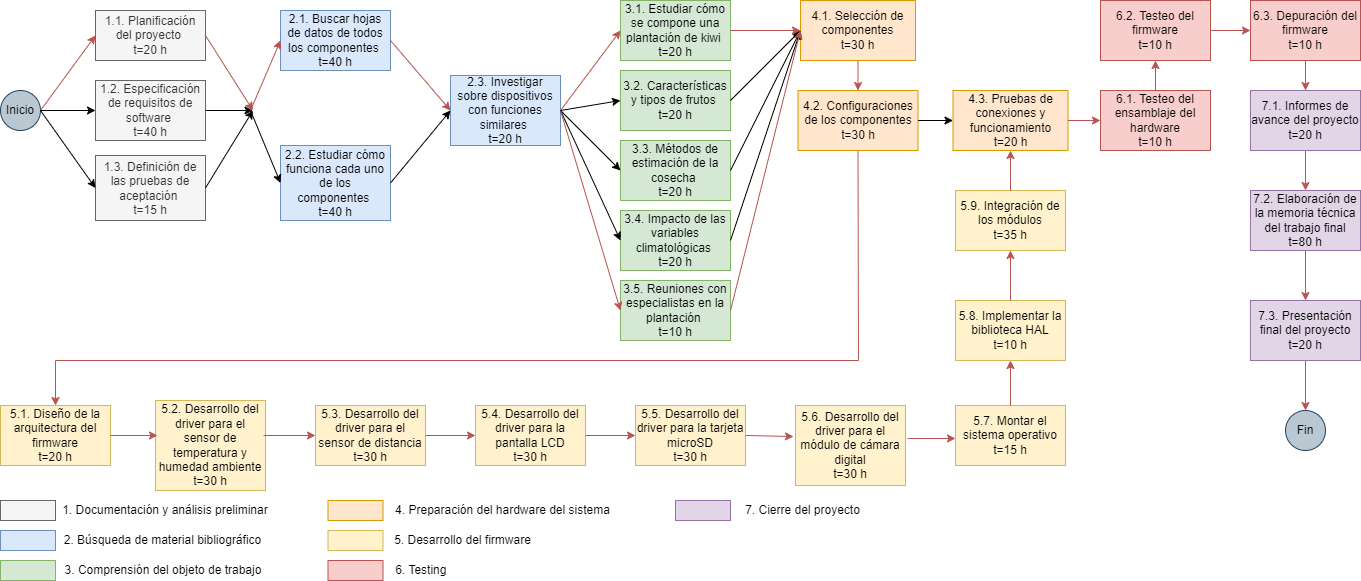
\includegraphics[width=24cm , height=11cm]{./Figuras/DAON.png}
\caption{Diagrama de \textit{Activity on Node}.}
\label{fig:DAON}
\end{figure}

\end{landscape}


\section{11. Diagrama de Gantt}
\label{sec:gantt}

En la figura \ref{fig:gantt} se muestra el diagrama de Gantt del proyecto. Para su realización se estableció un horario laboral de 6 horas de lunes a viernes.

\begin{figure}[htpb]
  \begin{center}
    \begin{ganttchart}[
      time slot unit=day,
      time slot format=isodate,
      x unit=0.038cm,
      y unit title=0.4cm,
      y unit chart=0.6cm,
      milestone/.append style={xscale=4}
      ]{2024-06-17}{2024-12-18}
      \gantttitlecalendar*{2024-06-17}{2024-12-18}{year} \\
      \gantttitlecalendar*{2024-06-17}{2024-12-18}{month} \\
      \ganttgroup{Duración Total}{2024-06-17}{2024-10-31} \\
      %%%%%%%%%%%%%%%%%Documentación y análisis preliminar
      \ganttgroup{Documentación y análisis preliminar}{2024-06-17}{2024-06-20} \\
      \ganttbar{Planificación del proyecto}{2024-06-17}{2024-06-20} \\
      \ganttbar{Especificación de requisitos de software}{2024-06-17}{2024-06-20} \\
      \ganttbar{Definición de las pruebas de aceptación}{2024-06-17}{2024-06-20} \\
      %%%%%%%%%%%%%%%%%Búsqueda de material bibliográfico
      \ganttgroup{Búsqueda de material bibliográfico}{2024-06-21}{2024-6-30} \\
      \ganttbar{Buscar hojas de datos de todos los componentes}{2024-06-21}{2024-6-27} \\
      \ganttbar{Estudiar cómo funciona cada uno de los componentes}{2024-06-21}{2024-6-27} \\
      \ganttbar{Investigar sobre dispositivos con funciones similares}{2024-6-28}{2024-6-30} \\
      %%%%%%%%%%%%%%%%%Comprensión del objeto de trabajo
      \ganttgroup{Comprensión del objeto de trabajo}{2024-07-1}{2024-7-4} \\
      \ganttbar{Estudiar cómo se compone una plantación de kiwi}{2024-07-1}{2024-7-4} \\
      \ganttbar{Características y tipos de frutos}{2024-07-1}{2024-7-4} \\
      \ganttbar{Métodos de estimación de la cosecha}{2024-07-1}{2024-7-4} \\
      \ganttbar{Impacto de las variables climatológicas}{2024-07-1}{2024-7-4} \\
      \ganttbar{Reuniones con especialistas en la plantación}{2024-07-1}{2024-7-2} \\
      %%%%%%%%%%%%%%%%%Preparación del hardware del sistema
      \ganttgroup{Preparación del hardware del sistema}{2024-07-5}{2024-9-3} \\
      \ganttbar{Selección de componentes}{2024-07-5}{2024-7-10} \\
      \ganttbar{Configuraciones de los componentes}{2024-07-11}{2024-7-15} \\
      \ganttbar{Pruebas de conexiones y funcionamiento}{2024-08-31}{2024-9-3} \\
      %%%%%%%%%%%%%%%%%Desarrollo del firmware
      \ganttgroup{Desarrollo del firmware}{2024-07-21}{2024-8-30} \\
      \ganttbar{Diseño de la arquitectura del firmware}{2024-07-21}{2024-7-24} \\
      \ganttbar{Desarrollo del driver para el sensor de temperatura y humedad}{2024-07-25}{2024-7-30} \\
      \ganttbar{Desarrollo del driver para el sensor de distancia}{2024-07-31}{2024-8-4} \\
      \ganttbar{Desarrollo del driver para la pantalla LCD}{2024-08-5}{2024-8-10} \\
      \ganttbar{Desarrollo del driver para la tarjeta microSD}{2024-08-11}{2024-8-15} \\
      \ganttbar{Desarrollo del driver para el módulo de cámara digital}{2024-08-16}{2024-8-20} \\
      \ganttbar{Montar el sistema operativo}{2024-08-21}{2024-8-22} \\
      \ganttbar{Implementar la biblioteca HAL}{2024-08-23}{2024-8-24} \\
      \ganttbar{Integración de los módulos}{2024-08-25}{2024-8-30} \\
      %%%%%%%%%%%%%%%%%Testing
      \ganttgroup{Testing}{2024-09-4}{2024-9-10} \\
      \ganttbar{Testeo del ensamblaje del hardware}{2024-09-4}{2024-9-6} \\
      \ganttbar{Testeo del firmware}{2024-09-7}{2024-9-8} \\
      \ganttbar{Depuración del firmware}{2024-09-9}{2024-9-10} \\
      %%%%%%%%%%%%%%%%%Cierre del proyecto
      \ganttgroup{Cierre del proyecto}{2024-09-11}{2024-10-3} \\
      \ganttbar{Informes de avance del proyecto}{2024-09-11}{2024-9-14} \\
      \ganttbar{Elaboración de la memoria técnica del trabajo final}{2024-09-15}{2024-9-29} \\
      \ganttbar{Presentación final del proyecto}{2024-09-30}{2024-10-3} \\
      %%%%%%%%%%%%%%%%%%%%%%%%%%%%%%%%%%%%%%%%%%%%%%%%%%%%%%%%%%%%%%%
    \end{ganttchart}
  \end{center}
  \caption{Diagrama de Gantt.}
  \label{fig:gantt}
\end{figure}


\section{12. Presupuesto detallado del proyecto}
\label{sec:presupuesto}

Los precios expresados en la siguiente tabla se encuentran en peso argentino (ARS) y fue estimado el 20 de mayo del 2024.

\begin{table}[htpb]
\centering
\begin{tabularx}{\linewidth}{@{}|X|c|r|r|@{}}
\hline
\rowcolor[HTML]{C0C0C0} 
\multicolumn{4}{|c|}{\cellcolor[HTML]{C0C0C0}COSTOS DIRECTOS} \\ \hline
\rowcolor[HTML]{C0C0C0} 
Descripción &
  \multicolumn{1}{c|}{\cellcolor[HTML]{C0C0C0}Cantidad} &
  \multicolumn{1}{c|}{\cellcolor[HTML]{C0C0C0}Valor unitario} &
  \multicolumn{1}{c|}{\cellcolor[HTML]{C0C0C0}Valor total} 
  \\ 
  \hline Tarjeta de desarrollo STM32F429ZI
 &
  \multicolumn{1}{c|}{1} &
  \multicolumn{1}{c|}{23 491} &
  \multicolumn{1}{c|}{23 491} 
  \\ 
  \hline Módulo Dht11 Sensor De Temperatura Humedad
 &
  \multicolumn{1}{c|}{1} &
  \multicolumn{1}{c|}{2 399} &
  \multicolumn{1}{c|}{2 399} 
  \\ 
  \hline Sensor Ultrasonico Hc Sr04
 &
  \multicolumn{1}{c|}{1} &
  \multicolumn{1}{c|}{2 300} &
  \multicolumn{1}{c|}{2 300}
  \\ 
  \hline Modulo Display Lcd 16x2 Con I2c
 &
  \multicolumn{1}{c|}{1} &
  \multicolumn{1}{c|}{5 785} &
  \multicolumn{1}{c|}{5 785}
  \\ 
  \hline Módulo Lector De Tarjetas Micro Sd
 &
  \multicolumn{1}{c|}{1} &
  \multicolumn{1}{c|}{3 600} &
  \multicolumn{1}{c|}{3 600}
  \\ 
  \hline Módulo cámara OV7670
 &
  \multicolumn{1}{c|}{1} &
  \multicolumn{1}{c|}{8 000} &
  \multicolumn{1}{c|}{8 000}
  \\ 
  \hline Kit 40 Cables Dupont
 &
  \multicolumn{1}{c|}{1} &
  \multicolumn{1}{c|}{2 712} &
  \multicolumn{1}{c|}{2 712}
  \\ 
  \hline Batería 3.7v 2000 mA
 &
  \multicolumn{1}{c|}{1} &
  \multicolumn{1}{c|}{15 205} &
  \multicolumn{1}{c|}{15 205}
  \\ 
  \hline Cable USB mallado
 &
  \multicolumn{1}{c|}{1} &
  \multicolumn{1}{c|}{5 300} &
  \multicolumn{1}{c|}{5 300}
  \\ 
  \hline Horas de ingeniería
 &
  \multicolumn{1}{c|}{725} &
  \multicolumn{1}{c|}{35 264} &
  \multicolumn{1}{c|}{25 566 400}
  \\ 
  \hline
\multicolumn{3}{|c|}{SUBTOTAL} &
  \multicolumn{1}{c|}{25 635 192} \\ \hline
\rowcolor[HTML]{C0C0C0} 
\multicolumn{4}{|c|}{\cellcolor[HTML]{C0C0C0}COSTOS INDIRECTOS} \\ \hline
\rowcolor[HTML]{C0C0C0} 
Descripción &
  \multicolumn{1}{c|}{\cellcolor[HTML]{C0C0C0}Cantidad} &
  \multicolumn{1}{c|}{\cellcolor[HTML]{C0C0C0}Valor unitario} &
  \multicolumn{1}{c|}{\cellcolor[HTML]{C0C0C0}Valor total} 
  \\ 
  \hline 30 \% de los costos directos
&
\multicolumn{1}{|l|}{1} &
\multicolumn{1}{|l|}{1} &
\multicolumn{1}{|l|}{7 690 558} 
   \\ \hline
\multicolumn{3}{|c|}{SUBTOTAL} &
  \multicolumn{1}{c|}{7 690 558} \\ \hline
\rowcolor[HTML]{C0C0C0}
\multicolumn{3}{|c|}{TOTAL} &
\multicolumn{1}{|l|}{33 325 750} 
   \\ \hline 
\end{tabularx}
\end{table}


\section{13. Gestión de riesgos}
\label{sec:riesgos}
En este apartado se mencionan los posibles riesgos del proyecto y el plan de mitigación.

a) Identificación de los riesgos y estimación de sus consecuencias:
 
Riesgo 1: demora para conseguir los componentes electrónicos requeridos.
\begin{itemize}
	\item Severidad (7): el proyecto sufrirá retrasos en su desarrollo.\\
	\item Probabilidad de ocurrencia (6): el mercado local no cuenta con el stock de los componentes necesarios para el proyecto.
\\
\end{itemize}   

Riesgo 2: daño o pérdida del hardware del proyecto.
\begin{itemize}
	\item Severidad (8): esto genera un retraso importante en la ejecución de las actividades del proyecto en la fase de implementación y pruebas.\\
	\item Ocurrencia (4): el encargado del proyecto será una persona muy cuidadosa y responsable.\\
\end{itemize}

Riesgo 3: mala estimación de la planificación.
\begin{itemize}
	\item Severidad (7): el proyecto sufrirá varios cambios y retrasos en la ejecución.\\
	\item Ocurrencia (8): no se cuenta con experiencia en planificación de proyectos.\\
\end{itemize}

Riesgo 4: variación de precios en la compra del hardware.
\begin{itemize}
	\item Severidad (8): el capital necesario para adquirir el equipo del proyecto se vería afectado.\\
	\item Ocurrencia (8): se tiene conocimiento de que existe mucha fluctuación en los precios de mercado.\\
\end{itemize}

Riesgo 5: retraso en la programación del firmware.
\begin{itemize}
	\item Severidad (8): retrasos en el proyecto debido a que el firmware es una parte fundamental en el momento de la integración e implementación del prototipo.\\
	\item Ocurrencia (7): falta de conocimiento y experiencia en la tecnología del hardware.\\
\end{itemize}

b) Tabla de gestión de riesgos:

\begin{table}[htpb]
\centering
\begin{tabularx}{\linewidth}{@{}|X|c|c|c|c|c|c|@{}}
\hline
\rowcolor[HTML]{C0C0C0} 
Riesgo & S & O & RPN & S* & O* & RPN* \\ \hline
Demora para conseguir los componentes electrónicos requeridos & 7 & 6 & 42  &    &    &      \\ \hline
Daño o pérdida del hardware del proyecto & 8 & 4 & 32  &    &    &      \\ \hline
Mala estimación de la planificación & 7 & 8 & \cellcolor{red}{56}  & 8  & 5  & \cellcolor{green}{40}   \\ \hline
Variación de precios en la compra del hardware & 8 & 8 & \cellcolor{red}{64}  & 9 & 5  & \cellcolor{green}{45}   \\ \hline
Retraso en la programación del firmware & 8 & 7 & \cellcolor{red}{56}  & 8  & 5  & \cellcolor{green}{40}   \\ \hline
\end{tabularx}%
\end{table}

Criterio adoptado: se tomarán medidas de mitigación en los riesgos cuyos números de RPN sean mayores a 45.

Nota: los valores marcados con (*) en la tabla corresponden luego de haber aplicado la mitigación.

c) Plan de mitigación de los riesgos que originalmente excedían el RPN máximo establecido:
 
Riesgo 3*: se consultará con el director la planificación para ajustar los tiempos de las tareas de acuerdo a su experiencia.
  \begin{itemize}
	\item Severidad (8): probabilidad que se modifiquen tiempos ya definidos a tareas.
	\item Probabilidad de ocurrencia (5): Se reduce el riesgo de hacer una mala planificación del proyecto.
	\end{itemize}

Riesgo 4*: se consultará con el cliente la posibilidad de efectuar compras de hardware con anticipación.
  \begin{itemize}
	\item Severidad (9): puede que el cliente no disponga de capital para hacer una compra anticipada.
	\item Probabilidad de ocurrencia (5): se reduce el riesgo de variación de precios.
	\end{itemize}

Riesgo 5*: Se dedicará más tiempo a la investigación de la tecnología y se buscará ayuda en algún ingeniero que haya desarrollado proyectos de estas características.
  \begin{itemize}
	\item Severidad (8): No cambia.
	\item Probabilidad de ocurrencia (5): Se obtendrá mayor conocimiento y experiencia en este tipo de tecnología.
	\end{itemize}


\section{14. Gestión de la calidad}
\label{sec:calidad}

Para cada uno de los requerimientos funcionales, a continuación, se lista su respectiva verificación y validación. Estas serán llevadas a cabo por el responsable del proyecto.

\begin{itemize} 
\item Req \#1.1: El sistema debe registrar la temperatura del ambiente.
\begin{itemize}
	\item Verificación: Revisar que el módulo realiza la toma de temperatura correctamente.
	\item Validación: Probar que se obtuvieron los valores del sensor mostrando los datos obtenidos en un monitor serial.
\end{itemize}
\end{itemize}

\begin{itemize} 
\item Req \#1.2: El sistema debe registrar la humedad del ambiente.
\begin{itemize}
	\item Verificación: Revisar que el módulo realiza la toma de humedad correctamente.
	\item Validación: Probar que se obtuvieron los valores del sensor mostrando los datos obtenidos en un monitor serial.
\end{itemize}
\end{itemize}

\begin{itemize} 
\item Req \#1.3: El sistema debe informar el espacio disponible de la tarjeta microSD.
\begin{itemize}
	\item Verificación: Revisar que el módulo realiza el registro de la información guardada.
	\item Validación: Conectar la tarjeta microSD en una computadora para comparar el espacio disponible con lo informado por el sistema.
\end{itemize}
\end{itemize}

\begin{itemize} 
\item Req \#1.4: El sistema debe informar la cantidad de fotos tomadas.
\begin{itemize}
	\item Verificación: Revisar si se guardan las fotografías en el medio de almacenamiento.
	\item Validación: Probar de contabilizar el total de fotos y mostrar el valor en un monitor serial.
\end{itemize}
\end{itemize}

\begin{itemize} 
\item Req \#2.2: El firmware debe estar modularizado.
\begin{itemize}
	\item Verificación: Comprobar si se armaron distintos módulos para cada dispositivo.
	\item Validación: Hacer funcionar cada módulo de manera aislada para ver los resultados obtenidos.
\end{itemize}
\end{itemize}

\begin{itemize} 
\item Req \#2.3: El firmware debe estar sobre un sistema operativo.
\begin{itemize}
	\item Verificación: Revisar el funcionamiento del sistema operativo.
	\item Validación: Realizar llamadas al sistema operativo y comprobar su respuesta.
\end{itemize}
\end{itemize}

\begin{itemize} 
\item Req \#3.4: La información en pantalla debe actualizarse cada 5 segundos.
\begin{itemize}
	\item Verificación: Revisar el funcionamiento de la pantalla LCD.
	\item Validación: Inspeccionar visualmente si la información mostrada es actualizada en el lapso de tiempo establecido.
\end{itemize}
\end{itemize}

\begin{itemize} 
\item Req \#4.1: Las fotos deben almacenarse en un formato de archivo JPG o JPEG.
\begin{itemize}
	\item Verificación: Revisar si la imagen está almacenada correctamente.
	\item Validación: Inspeccionar visualmente en una computadora si la imagen tiene la extensión de archivo esperada.
\end{itemize}
\end{itemize}

\begin{itemize} 
\item Req \#4.2: Las imágenes capturadas deben tener un mínimo de resolución de 640 x 480.
\begin{itemize}
	\item Verificación: Revisar si la imagen está almacenada correctamente.
	\item Validación: Inspeccionar visualmente en una computadora si la resolución de archivo es la esperada.
\end{itemize}
\end{itemize}

\begin{itemize} 
\item Req \#4.3: Cada imagen guardada no debe superar los 10 MB.
\begin{itemize}
	\item Verificación: Revisar si la imagen está almacenada correctamente.
	\item Validación: Inspeccionar visualmente en una computadora si el tamaño de archivo es el esperado.
\end{itemize}
\end{itemize}

\begin{itemize} 
\item Req \#5.2: Se debe presentar una memoria técnica al final del proyecto.
\begin{itemize}
	\item Verificación: Verificar que se haya presentado la memoria técnica del proyecto.
	\item Validación: Revisar que se cumplieron los requerimientos estipulados en el plan de proyecto.
\end{itemize}
\end{itemize}


\section{15. Procesos de cierre}    
\label{sec:cierre}
En esta sección se establecen las pautas de trabajo para realizar una reunión final de evaluación del proyecto, tal que contemple las siguientes actividades:

\begin{itemize}
	\item Pautas de trabajo que se seguirán para analizar si se respetó el Plan de Proyecto original:\\
    \begin{itemize}
        \item Encargado: \authorname
        \item Procedimiento: Se analizará el cumplimiento con los requerimientos y cronograma establecidos. En el caso de hallar requerimientos incumplidos y/o retrasos en las tareas se evaluarán las causas y se propondrán acciones para evitarlo en futuros proyectos.
    \end{itemize}
\end{itemize}

\begin{itemize}
	\item Identificación de las técnicas y procedimientos útiles e inútiles que se emplearon, y los problemas que surgieron y cómo se solucionaron:\\
    \begin{itemize}
        \item Encargado: \authorname
        \item Procedimiento: Se evaluarán los procedimientos utilizados en función a su utilidad y eficiencia para alcanzar los objetivos predefinidos. Se analizarán los problemas surgidos y las medidas paliativas.
    \end{itemize}
\end{itemize}

\begin{itemize}
	\item Indicar quién organizará el acto de agradecimiento a todos los interesados, y en especial al equipo de trabajo y colaboradores:\\
    \begin{itemize}
        \item Encargado: \authorname
        \item Procedimiento: Tras la exposición pública del proyecto frente al jurado, se llevará a cabo un expresivo reconocimiento hacia aquellos que contribuyeron a su realización, incluyendo al director del trabajo, los miembros del jurado y las autoridades de la CESE.
    \end{itemize}
\end{itemize}


\end{document}